\section{Procedure}\label{sec:procedure}
\subsection{Uniform plane waves in a parallel plate structure}
A perfect parallel plate wave guide is created in \mefisto by bounding a region of air with opposite, perfect electrical and magnetic boundaries.
The ends of the waveguide are covered with an absorbing boundary.
A wave source fills a vertical slice of the waveguide and will act on a transverse and parallel animation region.
This arrangement is shown in Fig. \ref{fig:waveguide}, with the bottom electrical boundary, animation regions and source present.

\begin{figure}[tbph]
	\centering
	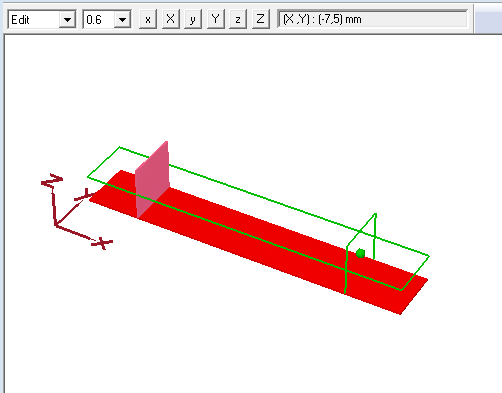
\includegraphics[width=0.7\linewidth]{graphics/waveguide}
	\caption{Perfect waveguide with dimensions 60 mm \by 10 mm \by 10 mm}
	\label{fig:waveguide}
\end{figure}

The source emits a wave with $f = \SI{15}{\giga\hertz}$ that travels through the medium, bounded by the walls of the waveguide.
The solid red color of the $yz$-animation plane in Fig. \ref{fig:Task1-2dsurface} shows that the wave travels as a plane wave from its origin through the waveguide.

\begin{figure}[tbph]
	\centering
	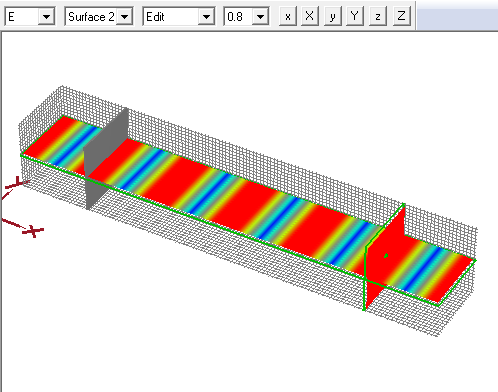
\includegraphics[width=0.7\linewidth]{graphics/Task1-2dsurface}
	\caption{Wave propagation in air-filled waveguide}
	\label{fig:Task1-2dsurface}
\end{figure}

The wave that is emitted from the source looks like a plane wave when we look at the small portion of it that is displayed in the y-z animation region. The solid red colour indicates an infinite plane wave. This agrees with the theory that a spherical wave can be approximated as a plane wave in the far field region as well as when looking at only a small portion of the wave. 

The physical properties of the propagation medium can be determined by examining the wave structure from Fig. \ref{fig:Task1-2dsurface}

\begin{figure}[tbph]
	\centering
	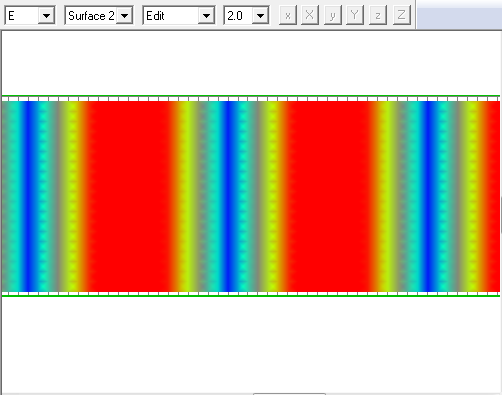
\includegraphics[width=0.7\linewidth]{graphics/Task1-scale}
	\caption{$xy$ view of propagation in Fig. \ref{fig:Task1-2dsurface}, with 0.5 mm mesh}
	\label{fig:Task1-scale}
\end{figure}

With this color scheme, blue regions indicate minima and maxima of the wave.
There are 20 grid square between adjacent blue regions in Fig. \ref{fig:Task1-scale}.
At 0.5 mm mesh resolution, this indicates that $\lambda = \SI{20}{\milli\meter}$.

\subsection{Waves in a non-ideal parallel plate structure}\label{sec:non-ideal}
Removing the magnetic sidewalls from the waveguide allows the wave energy to escape the confines of the guide.
When this change is made the wave propagation appears spherical near the source.
As the energy moves away from the source, the propagation becomes more planar.
This can be seen in Fig. \ref{fig:non-ideal}\subref{fig:3d}.
Fig. \ref{fig:non-ideal}\subref{fig:yz} shows that the orientation of all $\vec{E_z}$ are identical but their magnitude is not.

\begin{figure}[htpb]
	\centering
	\subfigure[]
	{
		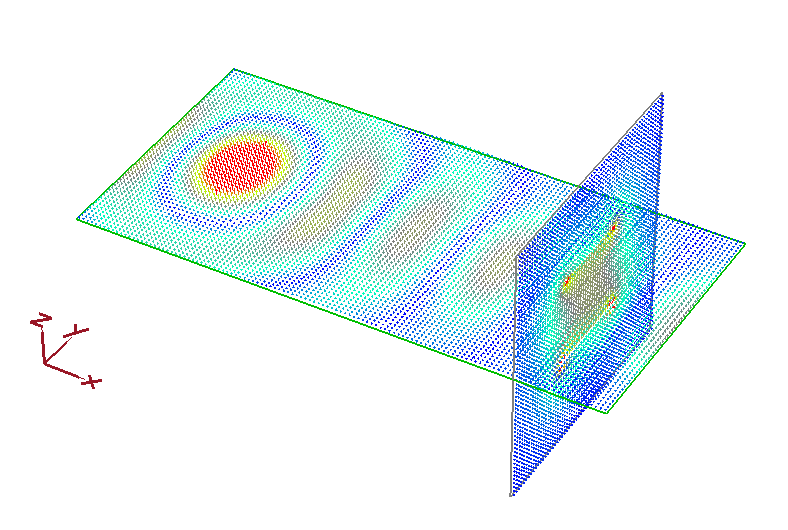
\includegraphics[width=0.575\linewidth]{graphics/Task2-3d-animation}
		\label{fig:3d}
	}
	\subfigure[$yz$-orientation]
	{
		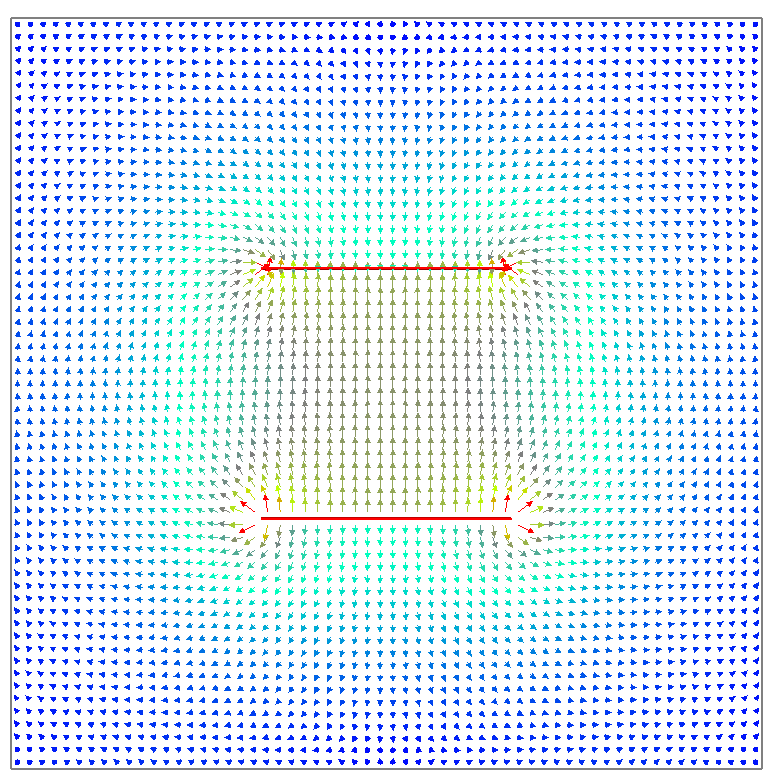
\includegraphics[width=0.375\linewidth]{graphics/Task2-yz-animation}
		\label{fig:yz}
	}
	\caption{Propagation in a non-ideal parallel plate}
	\label{fig:non-ideal}
\end{figure} 

\subsection{Dielectric and lossy media}\label{sec:dielectric}
The narrow-wide arrangement from Section \ref{sec:non-ideal} is changed to include a lossy dielectric between the top and bottom electric boundaries.
The boundaries with dielectric are shown in Fig. \ref{fig:plate-with-es}.

\begin{figure}[tbph]
	\centering
	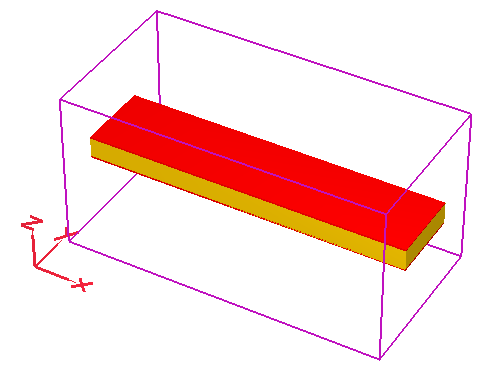
\includegraphics[width=0.7\linewidth]{graphics/plate-with-es}
	\caption{Waveguide containing a lossy dielectric material}
	\label{fig:plate-with-es}
\end{figure}

Propagation in the dielectric is shown in Fig. \ref{fig:Task3-3d-animation}.

\begin{figure}[tbph]
	\centering
	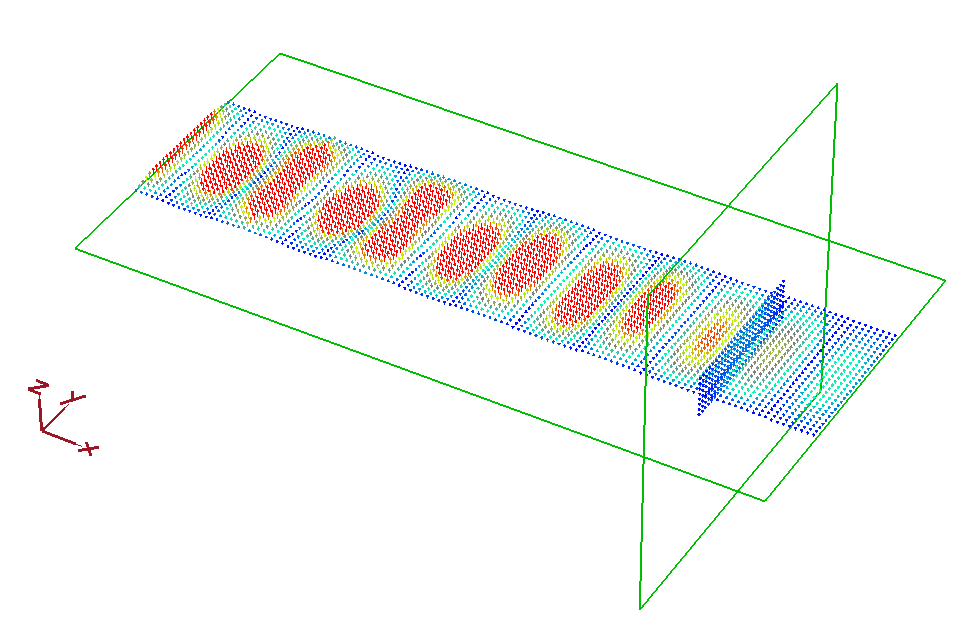
\includegraphics[width=0.7\linewidth]{graphics/Task3-3d-animation}
	\caption{Propagation in a waveguide filled with a dielectric where $\epsilon_r = 4$ and $\sigma = 0.5$}
	\label{fig:Task3-3d-animation}
\end{figure}

The wave attenuates as it travels through the waveguide as a result of $\sigma > 0$.
